\documentclass{article}

\usepackage{tikz}
\usetikzlibrary{shapes,arrows,calc,fit,backgrounds}
% Define a few styles and constants
\tikzset{sensor/.style={draw, rounded corners, text width=6em, text centered, minimum height=2.5em},
         box/.style = {minimum width=16pt,minimum height=16pt,draw},
         idles/.style = {very thick,draw=violet,text width=6em, align=center, minimum height=12em, rounded corners},
         line/.style = {,>=latex,->,draw=blue!50}}
\def\blockdist{4}
\def\tdist{2.25}

\begin{document}

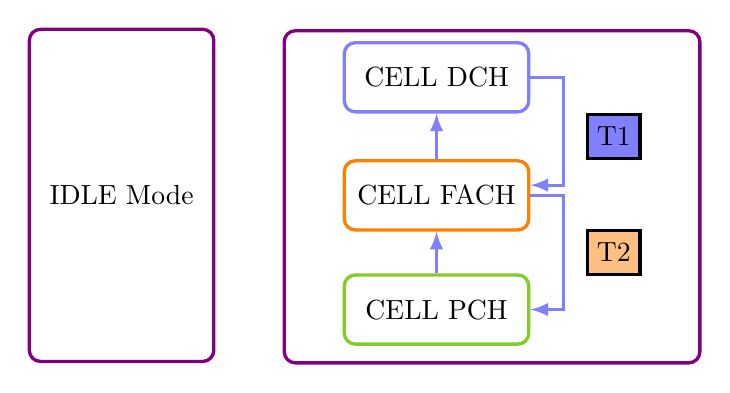
\begin{tikzpicture}[very thick]
\node (idle) [idles] {IDLE Mode};

\path ([yshift=1.5cm]idle)+(\blockdist,0) node [draw=blue!50] (dch) [sensor] {CELL DCH};
\path (idle)+(\blockdist,0) node [draw=orange] (fach) [sensor] {CELL FACH};
\path ([yshift=-1.45cm]idle)+(\blockdist,0) node [draw=yellow!50!green] (pch) [sensor] {CELL PCH};

% Draw connections between nodes
\draw [line] (dch.east) -- +(12pt,0) |- ([yshift=5pt]fach);
\draw [line] (fach.east) -- +(12pt,0) |- (pch);
\draw [line] (pch) -- (fach);
\draw [line] (fach) -- (dch);
\node (t1) [box,fill=blue!50] at ($(dch)!0.5!(fach)+(\tdist,0)$) {T1}; % You can create a style for the boxes used in this line and the next
\node (t2) [box,fill=orange!50] at ($(fach)!0.5!(pch)+(\tdist,0)$) {T2};

% Exercise: Discover how to place Connected Mode label
\begin{pgfonlayer}{background}
  \path (dch.west)+(-0.5cm,0.25cm) node (dchleft) {};
  \path (t2.east)+(0.5cm,0cm) node (t2right) {};
  \node [idles,fit=(dchleft) (pch) (t2right),draw] {};
\end{pgfonlayer}
\end{tikzpicture}
\end{document}
